Qui, di seguito, viene riportata l'architettura relativa alla prima solution. 

\lstinputlisting[language=C++]{solutions/s1/s1.cpp}

Si può notare come venga utilizzata una variabile temporanea \textit{ytmp} poiché essa viene utilizzata per calcolare l'uscita corrispondente. In particolare, il risultato calcolato ad ogni iterazione k viene sommato a quello della precedente iterazione. Pertanto, essendo che l'uscita deve essere solo assegnata e non letta per ogni iterazione, si utilizza una variabile temporanea per calcolare il risultato. Solo alla fine delle iterazioni si potrà assegnare il risultato all'uscita corrispondente. 

Effettuando la sintesi è possibile evidenziare il seguente report:\\
\begin{table}[H]
	\centering
	\begin{minipage}[t]{0.45\linewidth}
		\centering
		\begin{tabular}{|c|c|c|c|}
			\hline
			\textbf{Clock} & \textbf{Target} & \textbf{Estimated} & \textbf{Uncertainty} \\
			\hline
			ap\_clk & 10.00 & 8.510 & 1.25 \\
			\hline
		\end{tabular}
		\caption{HLS Solution 1 without Trip Count Timing Summary (ns)}
		\label{tab:hls-solution-1-timing-summary}
	\end{minipage}
	\hfill
	\begin{minipage}[t]{0.45\linewidth}
		\centering
		\begin{tabular}{|c|c|c|c|}
			\hline
			\multicolumn{2}{|c|}{\textbf{Latency}} & \multicolumn{2}{|c|}{\textbf{Interval}} \\
			min & max & min & max \\
			\hline
			? & ? & ? & ? \\
			\hline
		\end{tabular}
		\caption{HLS Solution 1 without Trip Count Latency Summary (clock cycles)}
		\label{tab:hls-solution-1-latency-summary}
	\end{minipage}
\end{table}

\begin{table}[H]
	\centering
	\begin{tabular}{|c|c|c|c|c|c|c|c|c|}
		\hline
		\multicolumn{1}{|c|}{Loop} & \multicolumn{2}{|c|}{\textbf{Latency}} & \multicolumn{1}{c|}{\textbf{Iteration Latency}} & \multicolumn{2}{c|}{\textbf{Initiation Interval}} & \multicolumn{1}{c|}{\textbf{Trip Count}}  \\
		Name & min & max &  & achieved & target &  \\
		\hline
		- loop1 & ? & ? & ? & - & - & 4 \\
		+ loop2 & ? & ? & 5 & - & - & ? \\
		\hline
	\end{tabular}
	\caption{HLS Solution 1 without Trip Count Latency Loops Summary}
	\label{tab:hls-solution-1-loop-summary}
\end{table}

Si può notare come la latenza associata a questa architettura risulta essere "?", cioè non definita. In particolare tale non definizione è dovuta al loop2 del quale non è definito il trip count associato essendo il numero di iterazioni corrispondente non noto a priori. Nello specifico, il ciclo 2 dipende dai valori presenti all'interno dell'array \textit{rowPtr} che sono incogniti poiché dipendono dai valori in input all'architettura. Viceversa, la latenza per ogni iterazione (IL), essendo che dipende dalla tipologia di operazioni, risulta essere definita. Per quanto riguarda, invece, il loop1, esso presenta un'iteration latency non definita poiché dipendente direttamente dal loop2 di cui non si è a conoscenza della latenza totale come spiegato precedentemente. Pertanto, la latenza totale del loop1 e, di conseguenza, la latenza totale associata all'architettura risulta essere non nota a priori. Quindi, per poter risolvere si specifica all'interno dell'implementazione la direttiva trip\_count. In particolare, si possono specificare tre valori all'interno di tale pragma: min, max e avg. Tali valori fanno riferimento rispettivamente al numero minimo, massimo e medio di iterazioni del loop di riferimento. In particolare, tenendo conto che in generale rowPtr[i] indica il numero di elementi non nulli al di sopra della i-esima riga all'interno della matrice, il loop2 è come se scandisse riga per riga la matrice. All'iterazione i del loop1 considera le iterazioni possibili all'interno del loop2 comprese tra il valore k=rowPtr[i] (corrispondente al numero di elementi non nulli presenti al di sopra della riga i) e il valore k=rowPtr[i+1] (corrispondente al numero di elementi non nulli presenti al di sopra della riga i+1). Quindi, la differenza tra rowPtr[i+1] e rowPtr[i] rappresenta il numero di elementi presenti all'interno della riga i. Pertanto, tale direttiva permette al tool di analizare come la latenza del loop contribuisce alla latenza totale dell'architettura così permettendo al progettista di effettuare ulteriori ottimizzazioni al design.

Pertanto, si allega l'architettura risultante.
\lstinputlisting[language=C++]{solutions/s1/s1tripcount.cpp}

Effettuando la sintesi è possibile evidenziare il seguente report:\\
\begin{table}[H]
	\centering
	\begin{minipage}[t]{0.45\linewidth}
		\centering
		\begin{tabular}{|c|c|c|c|}
			\hline
			\textbf{Clock} & \textbf{Target} & \textbf{Estimated} & \textbf{Uncertainty} \\
			\hline
			ap\_clk & 10.00 & 8.510 & 1.25 \\
			\hline
		\end{tabular}
		\caption{HLS Solution 1 with Trip Count Timing Summary (ns)}
		\label{tab:hls-solution-1-timing-summary}
	\end{minipage}
	\hfill
	\begin{minipage}[t]{0.45\linewidth}
		\centering
		\begin{tabular}{|c|c|c|c|}
			\hline
			\multicolumn{2}{|c|}{\textbf{Latency}} & \multicolumn{2}{|c|}{\textbf{Interval}} \\
			min & max & min & max \\
			\hline
			13 & 93 & 13 & 93 \\
			\hline
		\end{tabular}
		\caption{HLS Solution 1 with Trip Count Latency Summary (clock cycles)}
		\label{tab:hls-solution-1-latency-summary}
	\end{minipage}
\end{table}

\begin{table}[H]
	\centering
	\begin{tabular}{|c|c|c|c|c|c|c|c|c|}
		\hline
		\multicolumn{1}{|c|}{Loop} & \multicolumn{2}{|c|}{\textbf{Latency}} & \multicolumn{1}{c|}{\textbf{Iteration Latency}} & \multicolumn{2}{c|}{\textbf{Initiation Interval}} & \multicolumn{1}{c|}{\textbf{Trip Count}}  \\
		Name & min & max & & achieved & target &  \\
		\hline
		- loop1 & 12 & 92 & 3$\sim$23 & - & - & 4 \\
		+ loop2 & 0 & 20 & 5 & - & - & 0$\sim$4 \\
		\hline
	\end{tabular}
	\caption{HLS Solution 1 Latency with Trip Count Loops Summary }
	\label{tab:hls-solution-1-loop-summary}
\end{table}

Si può notare come, dopo aver applicato la direttiva di trip\_count, i valori di latenza risultano essere definiti numericamente. In particolare, il loop2 presenta un numero di iterazioni compresa tra 0 e 4, cioè rispettivamente il valore minimo e massimo specificati nel pragma di trip\_count. Bisogna ricordare che tale direttiva non ha impatto sull'architettura ma ha solo impatto sui cicli di latenza.

\begin{figure}[H]
	\centering
	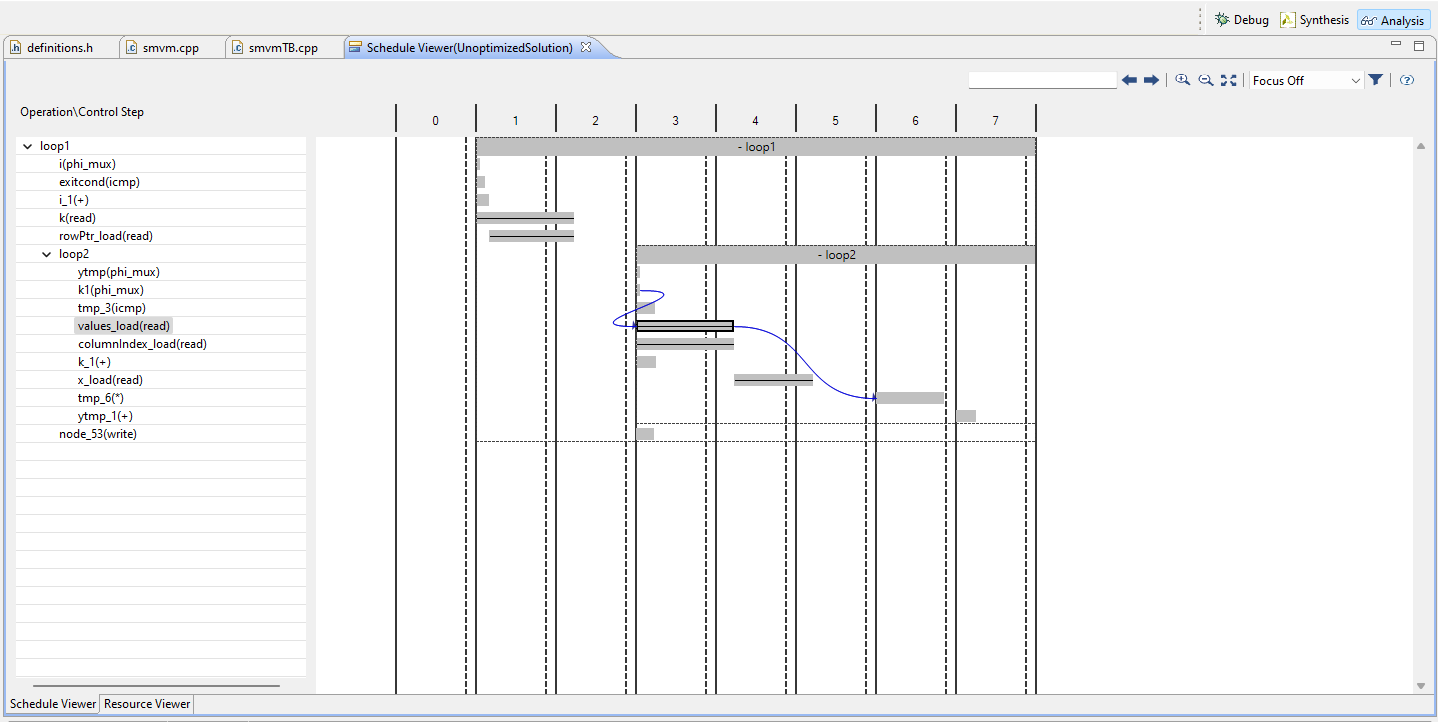
\includegraphics[width=0.9\textwidth]{solutions/s1/s1analysis.png}
	\caption{HLS Solution 1 Analysis}
\end{figure}

Qui di seguito, viene allegato l'utilizzazione delle risorse stimata dal processo di sintesi.
\begin{table}[H]
	\centering
	\begin{tabular}{|l|c|c|c|c|}
		\hline
		\textbf{Name}    & \textbf{BRAM\_18K} & \textbf{DSP48E} & \textbf{FF} & \textbf{LUT} \\ \hline
		DSP              & -                   & -               & -           & -            \\ 
		Expression       & -                   & 3               & 0           & 137          \\ 
		FIFO             & -                   & -               & -           & -            \\ 
		Instance         & -                   & -               & -           & -            \\ 
		Memory           & 0                   & -               & -          & -            \\ 
		Multiplexer      & -                   & -               & -           & 71          \\ 
		Register         & -                   & -               & 241         & -            \\ \hline
		\textbf{Total}   & 0                   & 3               & 241         & 208          \\ \hline
		\textbf{Available} & 280               & 220             & 106400      & 53200        \\ \hline
		\textbf{Utilization (\%)} & 0            & 1               & $\sim$0     & $\sim$0      \\ \hline
	\end{tabular}
	\caption{HLS Solution 1 with Trip Count Utilization Estimates Summary}
	\label{tab:hls-solution-1-utilization-estimates-summary}
\end{table}

Successivamente effettuando la C/RTL Cosimulation e l'Export RTL è possibile evidenziare i seguenti report.
\begin{table}[H]
	\centering
	\begin{tabular}{|c|c|c|c|c|c|c|c|}
		\hline
		\multicolumn{1}{|c|}{RTL} & \multicolumn{1}{|c|}{Status} & \multicolumn{3}{c|}{\textbf{Latency}} & \multicolumn{3}{c|}{\textbf{Interval}} \\
		&  & min & avg & max & min & avg & max \\
		\hline
		VHDL & Pass & 58 & 58 & 58 & NA & NA & NA \\
		\hline
	\end{tabular}
	\caption{HLS Solution 1 with Trip Count C/RTL Cosimulation Summary }
	\label{tab:hls-solution-1-cosimulation-summary}
\end{table}

\begin{table}[H]
	\centering
	\begin{minipage}[t]{0.45\linewidth}
		\centering
		\begin{tabular}{|l|r|}
			\hline
			\textbf{Resource} & \textbf{VHDL} \\
			\hline
			SLICE & 48 \\
			\hline
			LUT & 93 \\
			\hline
			FF & 161 \\
			\hline
			DSP & 3 \\
			\hline
			BRAM & 0 \\
			\hline
			SRL & 0 \\
			\hline
		\end{tabular}
		\caption{HLS Solution 1 with Trip Count Export RTL Resource Usage}
		\label{tab:hls-solution-1-export-rtl-resoruce-usage}
	\end{minipage}
	\hfill
	\begin{minipage}[t]{0.45\linewidth}
		\centering
		\begin{tabular}{|l|r|}
			\hline
			\textbf{Timing} & \textbf{VHDL} \\
			\hline
			CP required & 10.000 \\
			\hline
			CP achieved post-synthesis & 5.745 \\
			\hline
			CP achieved post-implementation & 5.692 \\
			\hline
		\end{tabular}
		\caption{HLS Solution 1 with Trip Count Export RTL Final Timing}
		\label{tab:hls-solution-1-export-rtl-final-timing}
	\end{minipage}
\end{table}